\documentclass[10pt,twocolumn]{article}

\usepackage{times}
\usepackage{fullpage}

\usepackage{booktabs}  % for \midrule
%\usepackage{subfigure}
\usepackage{balance}
\usepackage{graphicx}
\usepackage{xspace}
%\usepackage{pslatex}
%\usepackage{pifont}
%\usepackage{multirow}
%\usepackage{array}
%\usepackage{booktabs}
%\usepackage{cite}
\usepackage{url}
%\usepackage{cancel}
\usepackage{color,colortbl}
%\usepackage{microtype}
%\usepackage{textcomp}% http://ctan.org/pkg/textcomp
\usepackage{tabularx}
\usepackage{framed}
\usepackage[]{algorithm2e}
\SetAlFnt{\small}
\SetAlCapFnt{\small}
\usepackage{algorithmic}

\usepackage{listings}
%\usepackage{scrextend}
%\usepackage{mathtools}
\usepackage{pbox}
\usepackage{amsmath}

\let\labelindent\relax
\usepackage{enumitem}

\usepackage{tikz}
\usetikzlibrary{arrows,automata}
\usetikzlibrary{calc,positioning}
\usepackage{lipsum,adjustbox}


%\usepackage{tikz}
%\usepackage{decorations.pathmorphing}
%\usepackage{assymb}

\usepackage[labelfont=bf]{caption}

\usepackage{caption}
\usepackage{subcaption}
\usepackage{cleveref}
\captionsetup[subfigure]{subrefformat=simple,labelformat=simple}

%\theoremstyle{plain}
\newtheorem{theorem}{\bf{Theorem}}%[section]
\newtheorem{lemma}[theorem]{\bf{Lemma}}
\newtheorem{corollary}[theorem]{\bf{Corollary}}
\newtheorem{proofl}[theorem]{\bf{Proof}}
\newtheorem{proposition}[theorem]{\bf{Proposition}}

%\theoremstyle{definition}
\newtheorem{definition}{\bf{Definition}}%[section]
\newtheorem{observation}{\bf{Observation}}%[section] 

%\theoremstyle{remark}
\newtheorem{example}{\bf{Example}}
\newtheorem{notation}{\bf{Notation}}
\newtheorem{fact}{\bf{Fact}}

\usepackage{listings}
%%\usepackage{listings-golang}
\usepackage{color}

%\usepackage{sectsty}
%\sectionfont{\fontsize{12}{15}\selectfont}


\newcommand\mypara[1]{\vspace{.3em}\noindent\textbf{#1}}
\newcommand{\urlwofont}[1]{\urlstyle{same}\url{#1}}


%%%%%%%%%%%%%%%%%%%%%%%%%%%%%%%%%%%%%%%%
% Useful reviewing/feedback annotations
\input{annotations}
%%%%%%%%%%%%%%%%%%%%%%%%%%%%%%%%%%%%%%%%


\begin{document}

\title{Remote Memory Cuckoo Hashing}
%\author{WORDS '21 Submission \#3}
\author{Stewart Grant and Alex C. Snoeren\\ UC San Diego}
\date{}

\maketitle

\section*{Abstract}

Memory disaggregation promises high resource utilization,
and efficient resource sharing. However designing fully
disaggregated systems remains challenging due to the high
latency of remote memory. Key-value store indexes often
adopt a ~\textit{partially disaggregated} approach where
updates to the index are routed through a CPU for
serialization, while reads
 are made directly to memory.
Fully disaggregated indexes assume no such CPU and must
serialize updates entirely with remote clients.

This paper focuses on the design of a
 fully
 disaggregated
lock-based key-value index based on cuckoo
 hashing. Prior
work avoids locks in favor of optimistic concurrency as
locks can have large critical sections and quickly
bottleneck performance. However, optimistic approaches
require multiple round trips for each operation, as atomic
updates are limited to 64 bits with RDMA atomics. 

In this work we show that
with careful data structure and protocol design, as well as
the architecture of modern RDMA NICs traditional locking
strategies can perform better than state of the art
optimistic concurrency algorithms. We demonstrate this
through the design of a remote memory key value store based
on cuckoo hashing. Our cuckoo hashing algorithm (rcuckoo)uses dependent,
rather than independent hash functions to increase the
probability that both hashes of a key will be
close in the hash table. This locality enables fast lock
acquisition and release. We demonstrate that rcuckoo
outperforms optimistic concurrency algorithms by 2x in
terms of throughput and up to a 2x improvement on read
latency.

\section{Introduction}
\label{sec:intro}

%concurrent data structures round trips
Concurrent data structure design for remote memory is hard.
Access latency to remote memory is high so round trips per
operation must be minimized to achieve efficiency.
Serialization is particularly hard because there is no
centralized serialization point to guard access to remote
memory. RDMA NIC's provide atomic verbs such as
compare-and-swap (CAS), but these are by no means a silver
bullet.  Each atomic request takes a round trip from client
to server to execute. In the best case lock/unlock requires
two round trips, if multiple locks are required, or locks
are contested the number of round trips increases.

%cpu locking vs rdma
In traditional key-value stores (Memcached~\cite{memcached})
the CPU coordinates table access for read, write, and lock
instructions. In contrast RDMA based Key-value
stores~\cite{herd,erpc,pilaf} use a mixture of one-sided (no
cpu) and two-sided (cpu involved) verbs to alleviate the CPU
bottleneck. Reads are typically one sided to bypass the CPU
bottleneck~\cite{pilaf,cell} while writes are typically two
sided so memory-side CPU can orchestrate serialized
operations (e.g. locking) with main memory access latency
(50-100ns).  These small access times keep critical sections
small for CPU based locking, and dramatically increase them
for one-sided RDMA based locking schemes~\cite{clover,
sherman}.

%rdma and cuckoo hashing
In this work we examine the tradeoffs between optimistic and
lock based data structures for remote memory. Our
contribution is a new concurrent hash table design which
uses a novel cuckoo hashing algorithm. Our algorithm
(rcuckoo) is designed to enable locking and unlocking
efficiently using one-sided RDMA. In the common case our
reads execute in a single round trip, and updates to the
table are performed in two round trips. To achieve this
efficiency we make use of \textit{dependent hashing} to
increase the locality between hash location in our cuckoo
hash. Dependent hashing enables efficient reads, fast
heuristic search for open location, and efficient locking.
To achieve fast locking we make use of new RDMA NIC device
features, mainly RDMA masked CAS operations and device
mapped memory. Rcuckoo is designed with RDMA NIC's in mind
to achieve high throughput and low latency.

%%
Implement a prototype of our algorithm in python and
evaluate it in a simulator against another state of the art
remote hashing algorithm RACE. We demonstrate that in the
common case rcuckoo requires fewer round trips, and
therefore achieves lower latency and higher throughput than
race but up to a factor of 2x on YCSB workloads.
\section{Background}
\label{sec:background}

\subsection{RDMA}

\todo{this section needs to be crunched down}

\begin{figure*}[t]
    \centering
    \begin{subfigure}{0.3\linewidth}
        \includegraphics[width=0.99\linewidth]{fig/rdma_latency.pdf}
        % \label{fig:rdma_latency}
        % \caption{}
    \end{subfigure}
    \begin{subfigure}{0.3\linewidth}
        \includegraphics[width=0.99\linewidth]{fig/rdma_concur.pdf}
        % \label{fig:optimistic_failures}
        % \caption{}
    \end{subfigure}
    \begin{subfigure}{0.3\linewidth}
        \includegraphics[width=0.99\linewidth]{fig/rdma_cas_throughput.pdf}
        % \label{fig:optimistic_failures}
        % \caption{}
    \end{subfigure}
    \vspace{-1em}
    \caption{
    \textbf{(a)} CX5 RDMA latency vs message size~\cite{rdma-latency}
    \textbf{(b)} RDMA operation scalability
    \textbf{(c)} Compare and swap performance. Device memory vs main memory.
    }
    \label{fig:rdma-benchmarks}
\end{figure*}

RDMA is an enabling technology for memory disaggregation. It
allows client machines to directly access the memory of a
remote server with operations like read, write and atomic
update, without the involvement of a remote CPU (save for
initialization).  
%%
In the past decade the bandwidth
capabilities of RDMA NICs have increased disproportionately
to their latency improvement. The bandwidth difference
between CX3 and CX7 NICs is 10$\times$ and yet intra-rack
round trips of small RDMA packets has only shrunk by around
1.5$\times$.  Figure~\ref{fig:rdma-benchmarks}(a) shows the
tradeoff between NIC-to-NIC round trips times on CX5 RDMA
NICs for write operations. All packets up to 128 bytes have
comparable round trip latencies, and packet sizes must grow
to above 1K before the latency cost of a large packet
exceeds the cost of two round trips for smaller packets.
\textbf{If there is surplus bandwidth a single large message
can have much lower latency than two dependent smaller
messages}

RDMA verbs do not all have the same performance. Atomic
operations such as compare-and-swap (CAS) and fetch-and-add
(FAA) both have bottlenecks much lower than reads and
writes~\cite{design-guidelines,sherman}.
Figure~\ref{fig:rdma-benchmarks}(b) shows the scalability of
these operations on CX5 NICs for 64 bit operations.
%%
Atomic operations bottleneck due to PCIe round trips. 
Each operation issued from NIC to host memory requires a
PCIe round trip. Data dependent operations must queue until
the atomic operation completes.
%%
Vendors have recently provided a small region (256KB)
of device mapped memory which avoids the round trip on
atomic operations~\cite{device-memory}.
Figure~\ref{fig:rdma-benchmarks}(c) shows the relative
performance of CAS operation on device memory vs host
memory. Lock request on a single address are 3x higher
throughput, and independent lock requests scale at nearly
the same rate as read and write requests.

Additionally Mellanox provides non-standard verbs such as
64-bit masked compare-and-swap which sets individual bits in
a 64 bit word independently of unmasked
bits~\cite{rdma-masked-cas} This is useful for setting
multiple independent locks, assuming locks are close
together, as the state of all locks need not be known.


\subsection{RDMA Key-Value Stores}

%% %Describe existing key value stores relation to rdma and
%serialization %
Many non-disaggregated key-value stores have used RDMA to
accelerate their
performance~\cite{farm,memc3,erpc,herd,faast,mica,pilaf,cell,storm}.
%%
These systems strike a careful balance between directly
accessing memory with client side RDMA and serializing
requests with a server side CPU.
%%
Cuckoo and Hopscotch hashes have flourished in this space
because clients can locally calculate the location of keys
and perform lockless $O(1)$ reads with
RDMA~\cite{hopscotch,farm,pilaf,cuckoo}.
%%
Disaggregated key-value in contrast assume that a memory
server cannot provide serialization and orchestrate their
writes solely using
clients~\cite{rolex,fusee,clover,sherman,ford,race}. With
the exception of Sherman~\cite{sherman} these systems use
systems commit writes optimistically using 64 bit RDMA CAS. 
%%
Opportunistic writes have the advantage that updates are
atomically visible, no critical sections exist, and client
failures do not leave the table in an inconsistent state.
Unfortunately CAS based opportunistic writes perform poorly
under contention leading to high tail latencies
~\cite{clover}. Additionally RDMA CAS does not scale
well~\cite{design-guidelines}(Figure~\ref{fig:rdma-benchmarks}(b)),
and their small word width and lack of multi-CAS support
constrain the size and types of updates they can perform.

CAS width in particular effects system design because
key-value pairs can rarely fit into 64 bits, indexes updated
with CAS must reference keys values indirectly with a
pointer. At minimum resolving a remote pointer requires an
additional round trip for every read~\cite{race,clover}.
%%
As we will show in the following section data structures
like cuckoo and hopscotch hashes are difficult implement with
optimistic CAS updates because they require multiple updates
to execute atomically.


\subsection{Cuckoo Hashing} 
\label{sec:cuckoo-back}
Cuckoo hashing uses two independent hash functions to assign
keys a primary and secondary table location. When a key is
inserted if its primary location is occupied the existing
key is evicted to its alternative location. If the eviction
causes another collision the process iterates until an open
location is found. The path of evictions is known as
a~\textit{cuckoo path}. Cuckoo hashes use associative rows
to improve their maximum fill factors. In associative hashes
multiple clients can be chosen as eviction candidates and
breadth-first-search (BFS) has been shown to minimize both
cuckoo path length and critical section time~\cite{memc3,
cuckoo-improvements}.  While insertions require large
critical sections to perform search and execute updates
along the cuckoo path reads are executed in constant time by
reading both of a keys buckets~\cite{pilaf}.

%%now I want to explain why cuckoo hashing and disaggregation don't work well together.

Lockless $O(1)$ reads make Cuckoo hashing a desireable
candidate for a disaggregated index. However, long
unpredictable cuckoo paths and RDMA CAS limitations make
performing insertions without locks difficult in the
disaggregated setting. We designed an RDMA based cuckoo hash
to illustrate the difficulties of performing opportunistic
insertions. On inserts this system makes a sequence of reads
to calculate a valid cuckoo path and then itteratitivly
issues CAS operations to swap value along the path. If any
value on the path is concurrently modified by another client
the insertions will fail and must restart.
Figure~\ref{fig:cuckoo-problems}(a) shows how the failure
rate of insertions filling a table from 80-90\% full.

\textbf{Hopscotch Hashing} also enables fast reads by
localizing entries to a bounded range of addresses and we
considered using it as our core data structure. We believe
that although hopscotch hashing can likely be disaggregated
efficiently it is less straightforward than cuckoo hashing
for the following reasons:
%%
First, cuckoo insertions update one location per moved key while
hopscotch requires two. Hopscotch hashes keep a bitmask of
collisions per bucket which must also be updated when an
entry is relocated. Reno, a heavily one-sided RDMA hopscotch
hash, uses one sided atomics to sloppily update the bitmask
but requires a server side CPU to fix the bitmasks whenever
concurrent inserts execute~\cite{reno}. Both Farm and Reno
avoid ever executing long hopscotch chains because of their
execution time and complexity~\cite{farm,reno}.
%%
Second, an entries location in a cuckoo hash is easier to
predict than in hopscotch hashing which simplifies locking.
Cuckoo keys inhabit exactly one of two locations so locks
are predictable, conversely hopscotch locations occur on a
range so a locking strategy must lock the entire range
conservatively. Because each lock acquisition is expensive
this increases the fundamental difficulty of disaggregation
a hopscotch hash.
\section{Introduction}
\label{sec:intro}


\section{Background}
\label{sec:background}

\subsection{RDMA}

RDMA is a networking technology which allows client machines
to directly access the memory of a remote server. RDMA is an
enabling technology for memory disaggregation as
\textit{memory servers} do not need any computation
resources (save setting up the RDMA memory initially).

One sided RDMA verbs (read, write, atomic) are used to
access remote memory without any memory side computation.
One sided verbs require RDMA reliable connections which
guarantee in-order delivery of operations.

\subsection{Resource Disaggregation}

\subsection{Cuckoo Hashing}

%%path length and locking
A colision when inserting into a cuckoo hash table requires
displacing some number of keys. The sequence of displaced
keys called a \textit{cuckoo
path}~\cite{cuckoo-improvements}.


\subsection{Remote Memory Data Structures}

\section{Problems}
\label{sec:problems}

\begin{figure*}[t]
    \centering
    \begin{subfigure}{0.3\linewidth}
        \includegraphics[width=0.99\linewidth]{fig/optimistic_failures.pdf}
        % \label{fig:optimistic_failures}
        % \caption{}
    \end{subfigure}
    \begin{subfigure}{0.3\linewidth}
        \includegraphics[width=0.99\linewidth]{fig/optimistic_failures.pdf}
        % \label{fig:optimistic_failures}
        % \caption{}
    \end{subfigure}
    \begin{subfigure}{0.3\linewidth}
        \includegraphics[width=0.99\linewidth]{fig/optimistic_failures.pdf}
        % \label{fig:optimistic_failures}
        % \caption{}
    \end{subfigure}
    \vspace{-1em}
    \caption{
    \textbf{(a)} Failure rate of optimistic cuckoo insertions.
    \textbf{(b)} ~\todo{make}
    \textbf{(c)} ~\todo{make}
    }
    \label{fig:problems}
\end{figure*}

%concurrent data structures round trips
Concurrent data structure design for remote memory is hard.
Access latency to remote memory is high so round trips per
operation must be minimized to achieve efficiency.
Serialization is particularly hard because there is no
centralized serialization point to guard access to remote
memory. RDMA NIC's provide atomic verbs such as
compare-and-swap (CAS), but these are by no means a silver
bullet.  Each atomic request takes a round trip from client
to server to execute. In the best case lock/unlock requires
two round trips, if multiple locks are required, or locks
are contested the number of round trips increases.

%cpu locking vs rdma
In traditional key value stores (Memcached~\cite{memcached})
the CPU coordinates table access for read, write, and lock
instructions. In contrast RDMA based Key-value
stores~\cite{herd,erpc,pilaf} use a mixture of one-sided (no
cpu) and two-sided (cpu involved) verbs to alleviate the CPU
bottleneck. Reads are typically one sided to bypass the CPU
bottleneck~\cite{pilaf,cell} while writes are typically two
sided so memory-side CPU can orchestrate serialized
operations (e.g. locking) with main memory access latency
(50-100ns).  These small access times keep critical sections
small for CPU based locking, and dramatically increase them
for one-sided RDMA based locking schemes~\cite{clover,
sherman}.

\textbf{Caching:} Modifying a remote data structure requires
clients to have synchronized caches. The cache can either be
accumulated per operation and be discarded or persist across
operations.  Accumulating a cache per operation is slow,
clients must aquire locks, read, then release potentially
many times to complete an operation if the locks are fine
grained. Alternatively clients can persist a cache across
requests in the hope that it will be valid for future
operations.  Clover (a remote memory key value store) caches
pointers to values on clients to enable fast reads when
values are looked up multiple times~\cite{clover}.
Optimistic caching threads a fine line as issuing optimistic
operations which commonly fail may be worse than acquiring
the correct locks.  An ideal caching strategy would enable
clients to succeed in their operations frequently while not
requiring much overhead to maintain. 



%cuckoo hashing optimistic vs locks
\textbf{Critical Sections:} Consider executing an insert
into a concurrent cuckoo hash stored in remote memory. A
client with a cached index may have little or very stale
information about the state of the hash table. To insert the
client must gather information by reading buckets to compute
a cuckoo path. With concurrent clients this leads to a
chicken and egg problem when acquiring locks vs making
reads.

%% optimistic inserts
A client can perform inserts opportunistically by executing
lockless read to learn about the hash table, calculating a
cuckoo path, and executing a sequence of dependent CAS
operations for each step in the path. This approach is
scalable as its critical section is only the length of a CAS
instruction and is only limited by RDMA atomic operation
throughput~\cite{design-guidelines}. However, Paths can
become invalid as other clients running concurrent inserts
invalidate the paths. Figure~\ref{fig:problems}(a) shows the
path insertion failure rate as the number of concurrent
clients grows. This approach minimizes round trips as
dependent CAS operations can be batched thanks to in order
delivery provided by RDMA reliable connections.
Unfortunately failed inserts require additional round trips
to both fix the state of the table, and retry the
insert.\sg{Further - Issuing CAS as a batch leads to complex
path failure cases such a single element in the path failing
while others further down the path succeed. Assesing and
fixing such insertion failures without locks is very hard.}

% lock based inserts
Alternatively to get synchronized information the client can
lock the table, then issue reads. However acquiring locks
without knowledge of the table is hard. A global lock
ensures that all reads are synchronized, but bottlenecks
hash table throughput. Alternatively per bucket locks
enable high throughput but calculating which buckets to lock
requires knowledge of the table. A long cuckoo path may
require locking many buckets and many round trips to gather
information about the hash table.
%%
An ideal protocol would enable clients to perform inserts
without bottlenecks the insert performance of the hash
table, while requiring the fewest round trips to construct
and execute the cuckoo path.

% First, acquiring a lock means a round trip. If the table has
% a single lock, then a client is guaranteed to be able to
% gather all the locks it requires in a single round trip.
% However a single lock does not scale as only a single writer
% can write at a time. This matter is made worse by the fact
% that the critical section of the lock is larger in remote
% memory. Breaking the table up into subtables each with it's
% own lock has it's own problems. An insertion with a long
% path will potentially need to acquire many locks. Each of
% which requires a round trip. Therefore using fine grained
% locking increases the tables scalability but increases it's
% base case insertion time.

\textbf{Read Optimization:} Most data center workloads are
read heavy, therefore read operations should be the most
highly optimized~\cite{datacenter-workloads}. Prior
approaches such as RACE require two RDMA round trips per
read. The first is a hash index lookup, the second round
trip reads the actual key-value block. RACE must perform two
round trips because entries in the hash index are limited to
64 bits (CAS width). This is commonly not enough to store
both key and value so RACE can not inline both keys and
values in the index structure. Clover~\cite{clover} enables
single round trips reads. However under contention Clovers
reads require pointer chasing which is known to be expensive
due to each pointer resolution requiring a round
trip~\cite{clio,clover,pointer-chaising}. Ideally we would
be able to ensure that reads complete in a single round
trip.

\textbf{Duplicate Keys:} Clients may issue concurrent
inserts for the same key, given that keys may occupy
multiple location detecting and dealing with duplicate keys
is tricky while maintaining high performance. RACE requires
an extra round trip after each insert to check if a
duplicate key was inserted simultaneously~\cite{race}. An
ideal algorithm would prevent key duplication without
requiring additional overheads.


\section{Design}
\label{sec:design}

\subsection{Locality Hashing}
\begin{figure*}[t]
    \centering
    \begin{subfigure}{0.3\linewidth}
        \begin{align*}
            L_1 &= h_1(k) \\
            L_2 &= L_1 + h_2(k) \% f^{f + log_2(h_3(k))}
        \end{align*}
        % \caption{}
        \label{fig:hash_factor}
    \end{subfigure}
    \begin{subfigure}{0.3\linewidth}
        \includegraphics[width=0.99\linewidth]{fig/hash_factor.pdf}
        \label{fig:hash_factor}
        % \caption{}
    \end{subfigure}
    \begin{subfigure}{0.3\linewidth}
        \includegraphics[width=0.99\linewidth]{fig/hash_fill.pdf}
        \label{fig:hash_fill}
        % \caption{}
    \end{subfigure}.
    \vspace{-1em}
    \caption{
    \textbf{(a)} Dependent hashing for factor $f$.
    \textbf{(b)} CDF of distances between cuckoo locations dependent hashing on different exponential factors.
    \textbf{(c)} Exponential factor relation to max fill in cuckoo hash.
    }
    \label{fig:locality-hashing}

\end{figure*}


\begin{figure*}[t]
    \centering
    \begin{subfigure}{0.3\linewidth}
        \includegraphics[width=0.99\linewidth]{fig/rdma_latency.pdf}
        \label{fig:rdma_latency}
        % \caption{}
    \end{subfigure}.
    \begin{subfigure}{0.3\linewidth}
        \includegraphics[width=0.99\linewidth]{fig/insertion_span.pdf}
        \label{fig:insertion_span}
        % \caption{}
    \end{subfigure}.
    \begin{subfigure}{0.3\linewidth}
        \includegraphics[width=0.99\linewidth]{fig/buckets_per_lock_vs_locks_per_message_copy.pdf}
        \label{fig:tbd}
        % \caption{}
    \end{subfigure}.
    \vspace{-1em}
    \caption{
    \textbf{(a)} CX5 RDMA latency vs message size~\cite{rdma-latency}
    \textbf{(b)} CDF of cuckoo spans for dependent and independent hashing. A cuckoo span is the distance between the smallest and largest index in a cuckoo path.
    \textbf{(c)} Round trips required for locking with different lock configurations and locality hashing (99th percentile) - locks per message and buckets per lock.
    }
    \label{fig:rdma}

\end{figure*}


Both cuckoo~\cite{cuckoo} and hopscotch~\cite{hopscotch}
hashes are optimized for reads. Cuckoo hashing ensures
constant time reads, while hopscotch hashing ensures that a
read is within a bounded range of it's hash index. Both of
these properties have been noticed by the RDMA key-value
store, and far memory communities for their fast
reads~\cite{memc3,cuckoo-improvements,pilaf,farm}.

Our approach aims to combine the bounded reads of cuckoo
hashing, with the locality properties of hopscotch hashing.
To do so we bound the distance between cuckoo hash
locations. Figure~\ref{fig:rdma}(a) shows the tradeoff
between message size and latency for a ConnectX-5 RDMA NIC.
The latency of small messages (2-128 Bytes) are nearly
identical, and the size of a message must be larger than 1K
before it's latency is 2x that of a small message. Bandwidth
is increasingly available in modern networks with 800Gbps on
the horizon, we tradeoff bandwidth for latency by opting for
larger single messages and fewer round trips. In essence we
make large sloppy reads, and leave it to the client to
reconstruct a result.

Traditional cuckoo hashing calls for two independent hash
functions. We instead make our two hash functions
\textit{dependent}. The first hash function determines the
location a key will be hashed to. The second hash function
determines the maximum distance the second value can have
from the first. A third hash function determines a random
location between the first location, and the bound imposed
by the second. Figure~\ref{fig:locality-hashing}(a) shows
the formula for our dependent hashing function.

A strawman implementation of locality based hashing would
use the first hash function to find a location, and the
second to find a random location within a fixed bound. This
approach quickly leads to failed insertions. Due to the
birthday paradox the probability of a collision is high, and
on large tables the probability that one region of the hash
table will become full, and have not viable path to an open
slot is high. ~\todo{Insert a figure of one of my failed
insertion experiments on a big table}.

Rather than use a static bound we use a dynamic logarithmic
bound with a third hash function. The bound set by the
third hash function is determine by counting the suffix
zeros of the resultant hash and rasing it by an exponential
factor. In the common case the bound is small, but on an
exponentially decrease rate some pairs of values are spaced
far apart. This design enables some pairs to act
as~\textit{waypoints} to other regions of the table. This
method, paired with associative in the cuckoo hash enables
high fill rates while keeping the region of the table any
given key can inhabit small.

The tradeoff between the exponential factor and the mean
distance is fill factor.
Figure~\ref{fig:locality-hashing}(b) illustrates how
increasing the exponential factor shifts the distribution of
distances between cuckoo hash locations.
Figure~\ref{fig:locality-hashing}(c) shows how these same
factors effect the max fill rate of the table before an item
cannot be inserted.


\subsection{Locking}

Traditional wisdom would suggest that because cuckoo hashing
can have long insertion paths it is a poor candidate for
remote memory. Augmenting an insertion path requires making
many modifications to the hash table. There are two
approaches for making path modifications. The first is to
perform a set of compare and swap modification which migrate
an open slot down a path to a location where the new value
is inserted. In this case the client acquires no locks,
however it has no guarantee that it's insertion path with
remain valid as concurrent processes can modify the hash
table with insertions of their own. In this case the client
can opportunistically attempt an insertion path using its
cached information about the table. This strategy has the
potential to fail frequently, and the requires potentially
many reads to be issued for the client to keep it's path
information up to date. ~\todo{insert a plot which shows
path lengths and failure rates from the cukoo approach with
no batching.}

Alternatively a client can aquire locks for the table. Locks
typically have poor performance for disaggregated algorithms
because each lock and unlock operation requires a round
trip. This means that any locking algorithm will have a lock
acquisition phase in which all required locks are collected,
followed by a critical section in which the operations are
executed, and a lock release stage. Using a course grained
locks this approach leads to throughput bottlenecks as it
does not scale with the number of clients. However course
grained locks have the advantage that there are few locks to
aquire, therefore a lock acquisition and release algorithm
takes less round trips. A typical lock acquisition policy
works by acquiring locks in a predefined incremental order to
avoid deadlock. The tradeoff between fine grained and course
locking is clear - fine grained locking allows higher
degrees of parallelism and throughput, while adding higher
latency due to a more complex lock aquire and release stage.
Course locking has lower latency aquire and release, but
limits throughput as many clients will contest the same
locks.

Locality hashing enables very efficient locking due to RDMA
masked CAS
operations~\cite{advanced-transport,scalable-locks}. Without
local hashing fine grained locks would be scattered
throughout the hash table. Locality hashing increases the
probability that an insertion path is within a bounded
region of the hash table.  This means that a lock table with
lock locations corresponding to physical locations in the
hash table will be near one another.  
%%
Figure~\ref{fig:rdma}(b) shows the insert span in buckets
using both dependent and independent hashing on a table with
500K entries and 8 entry buckets. A span is calculated as
the distance between the lowest index and the highest index
in a cuckoo path. Past 50\% independent hashing spans a
random range in the table (whenever a displacement occurs on
insert). With dependent locality based hashing 95\% of
inserts span less than 32 buckets, and 99\% less than 256.
%%
RDMA masked CAS operations allow a client to set a 64 bit
mask along with the new, and old values of the cas
operation. This enables the client to atomically set up to
64 contiguous locks. Using these operations clients can
dramatically decrease the number of round trips required to
acquire locks.
%%
Lock granularity effects performance under contention. Using
values from Figure~\ref{fig:rdma}(b) if locks are per bucket
96\% of lock acquisitions can be completed with a single RTT
masked cas. If locks span 4 buckets 99\% of requests can be
completed in a single round trip.
%%
Figure~\ref{fig:rdma}(c) Shows the tradeoff between lock
granularity and the number of locks which can be set in a
single message with locality hashing turned on. The values
reported are the 99th percentile number of round trips
required to acquire locks up to a 90\% fill factor on a
table with 4096 entries and 8 entries per bucket, and 8
concurrent clients. The biggest factor in round trip times
is the number of locks per bucket. On the far right side of
the heatmap (512) only a single global lock exists. Further
the benefit in terms of locks per message falls off quickly
after 1. RDMA masked CAS are beneficial as they allow for
fine grained locking, but setting 3 or more locks per
message has little effect up to 90\% fill rate.

RDMA atomic throughput is
limited~\cite{design-guidelines}~\todo{[swordbox]}. Reducing
the number of atomic messuages also reduces hardware
limitations on the number of operations. Our lock table is
also small in compairision to the true hash table, each lock
is a single bit, and bits can correspond to multiple rows of
the table if we need to save space~\todo{lock size, vs locks
per message figure}. Because we can save lock space due to
masked cas we can also make use device mapped memory for
faster lock aquisition~\cite{sherman}. RDMA device mapped
memory reduces request latency by executing RDMA operations
onto memory which resides on the RDMA NIC. This memory is
highly constrained~\todo{4MB CX5,CX6}, it removes the need
for a PCIe round trip thereby reducing lock aquisition
latency by aproximatly 2x.


\subsection{Protocol}

Using locks instead of opportunistic concurrency greatly
reduces the round trips required to perform operations.
Insertions into a cuckoo hash require one message for each
entry in the cuckoo path. Executing the insertion
opportunistically with CAS operations enables concurrent
reads, and insertions, but each swap along the path is
blocking as it requires the prior CAS to complete. The round
trips required to perform an opportunistic search is tied to
the length of the cuckoo path. Further as inserts can run
concurrently path insertions can fail. A single failed
insert along the cuckoo path requires the client to stop and
retry it's insert. Alternatively using locks to guard
buckets can guarantee that cuckoo paths can be executed
without failure. Therefore all cuckoo path swaps can be
batched together into a single round trip.

Clients need their caches to be synchronized with the remote
hash table in order to generate correct cuckoo paths. We
batch reads with RDMA masked CAS operations to synchronize
their caches. When a lock request is issued a single read
which spans the range of the lock request is generated. The
read is issued after the lock request, although the two are
batched together. RDMA reliable connections ensure that on a
single QP operations are executed in order. Therefore if the
lock request returns successfully the batched read will
return synchronized values from the hash table which will
remain unmodified while the lock is held.

Clients with synchronized reads can generated cuckoo paths
which are guaranteed to be valid with lock search.
Therefore, all cuckoo path updates can be issued in a single
batch. Further, CAS operations can be swapped with writes.
Writes have higher throughput than CAS, and slightly lower
latency. We add checksums to our table entries to enable
concurrent reads~\cite{pilaf,cell}.  ~\todo{insert RDMA
benchmark for writes and cas.}

Given this propery our protocol for lock aquisition is as
follows. The client performs a search on its local cache for
an insertion path. A set of locks required for the insert
are generated. The locks are broken into a sequence of RDMA
masked CAS operations. Reads which span the range of each
locked bucket are generated alongside the maksed CAS
operations. Clients issue the lock request and the read
behind it. Once the locks are aquired and the reads are
received the clients cache is up to date.

The insertion path the client used to aquire locks may be
invalid after the lock have been aquired. The client
performs a second search for an insertion path only
searching entries from buckets it has locked. If a path
exists the client generates a sequence of write requests,
and unlock requests. The client issues writes and unlocks in
a batch. This read-lock, search, write-unlock pattern along
with locality hashing ensures that in most cases insertions
(as well as deletes and updates) are performed in two round
trips.

Our protocol saves round trips in comparison to RACE, which
uses three round trips in the common case. On inserts RACE
must re-read the hash table to ensure that concurrent CAS
operations did no insert duplicates. With our algorithm we
can simply check for duplicates by reading both insertion
hash locations when acquiring locks. On updates RACE must
read the index, then the data, and then perform the update
as the index is not large enough to store the key. 

RACE requires that each hash table index is 64 bits so it
can be atomically modified by a CAS. Because we use locks
our index can store larger entries containing the key. It
further enables us to store values in the index enabling
single RTT reads. This strategy increase our common case
read size in excahnge for latency~\todo{evaluation section}.
This same pattern is true in RACE for deletes. 
\todo{insert protocol message figure}

\textbf{Key Duplication:} Unlike RACE our algorithm can
prevent duplicate keys easily on insert. Cuckoo hashing
inserts to exactly one bucket, which is read during the lock
acquisition phase. If a duplicate key is found the client
can abort. If the bucket is full, a duplicate key may exist
in it's alternative bucket. Our clients issue a read to the
inserted keys alternative bucket during lock acquisition. If
the lock returns successfully and no duplicate exists in
either bucket then no duplicates exist as the successful
lock ensures that no other client is currently moving the
key to another location as part of a concurrent insert.

\subsection{Search}
Cuckoo hashing insert traditionally uses random
replacement~\cite{cuckoo}. Random replacement requires
little computation, however at high fill rates it leads to
long cuckoo paths which require many locks, and reduce
concurrent throughput. BFS search finds the shortest path
and has been demonstrated to increase system throughput with
fine grained locking~\cite{algorithmic-improvements}.

BFS search is computationally intensive. Locality based
hashing enables us to leverage more efficient search
strategies. Because locality hashing increases the
probability that a cuckoo hashing location is close we can
use an informed search algorithm to find open slots close to
bucket a key hashes to. 

In the case of BFS the target bucket is unknown, therefore
all paths must be explored. We use A* search, an algorithm
which takes a goal location, and a distance heuristic as
input. A* is known to find shortest paths in much better
average case times than BFS. A* requires two additional
inputs, a distance heuristic and a goal location.

\textbf{goal location}: Locality hashing increases the
probability that an open slot near the insertion target
location can terminate a cuckoo path. Our algorithm collects
open slots near the original hash location as candidate goal
locations. By default we set the number of candidate goal
locations to 5. Gloal locations are collected by starting at
the $h_1(k)$ location and iterating through the hash
table both forward and backwards through the table one index
at a time. Buckets with open slots are added to the
candidate list until the limit is reached. \todo{I could
improve this search time by tracking the list of open
buckets and using binary search on them.}.

\textbf{Search Heuristic}: A* requires a heuristic for
distance which is a strict underestimate of the true
distance to a goal. A typical heuristic for search is the
euclidean distance between two points. A * guarantees that
if the search heuristic is a strict underestimate of the
true distance to the goal then the path found will be the
shortest path. In our case we use the distance between a
goal state and a current state is unknown as the distance
between any two buckets is the result of our locality
hashing function which has no upper bound. However we can
estimate the distance between two buckets by using the mean
distance of our locality hash function. This approach does
not guarantee that we find the shortest path, however it
does find short paths in the common case, and results in
very short search times.


\section{Evaluation}
\label{sec:eval}

\section{Conclusion}
\label{sec:conclusion}

\section{Problems}
\label{sec:problems}

Designing a fully disaggregated shared index is difficult
because of high access latency. Operations which require
synchronization or blocking are amplified by the latency. As
a result minimizing round trips is critical to achieving low
latency per operation. These challenges are most pronounced
when synchronizing caches, and executing critical sections.


\textbf{Caching:} Modifying a shared structure from remote
clients requires cache synchronization. Opportunistic
updates speculate on the state of the unified cache while
pessimistic updates acquire locks then read, write, and
unlock. Porting prior cuckoo hashing algorithms to remote
memory directly would result in poor performance as clients
iteratively read one bucket at a time during search and then
aquire locks~\cite{cuckoo-improvements, memc3, pilaf}.
Determining how to accumulate a clients cache to perform an
insert in the fewest number of round trips is a key
challenge in building a remote cuckoo hash table.

% Accumulating a cache per operation is slow,
% clients must aquire locks, read, then release potentially
% many times to complete an operation if the locks are fine
% grained. Alternatively clients can persist a cache across
% requests in the hope that it will be valid for future
% operations.  Clover (a remote memory key value store) caches
% pointers to values on clients to enable fast reads when
% values are looked up multiple times~\cite{clover}.
% Optimistic caching threads a fine line as issuing optimistic
% operations which commonly fail may be worse than acquiring
% the correct locks.  An ideal caching strategy would enable
% clients to succeed in their operations frequently while not
% requiring much overhead to maintain. 


\textbf{Critical Sections:} Designing a fast, and fine
grained critical section for updates is a main challenge. As
a strawman consider an opportunistic approach to cuckoo
hashing. When a client wants to insert it iteratively reads
the remote index constructing a cuckoo path. Once an open
slot is found it executes a series of CAS operations to
perform the insert. If one element along the path is updated
the entire update will fail.
Figure~\ref{fig:cuckoo-problems}(a) shows the path insertion
failure rate as the number of concurrent clients grows using
this approach on a table with 10k entries filled to 90\%.
The failure rate of operation grows to over 80\% with each
failure requiring the algorithm to restart.

A naive lock based approach suffers from an inverse problem.
Using a single global lock all updates will succeed however
given a latency of 2us and two round trips to lock and
unlock, the theoretical limit of such an approach is 250k
operations per second, which in practice is much lower. As
such any lock based approach must used fine grained locks.
Acquiring multiple locks demands a deadlock free algorithm
in which each atomic acquisition must be performed in order.
This challenge makes is difficult to aquire many locks
efficiently as acquiring many locks far apart in memory
requires many round trips.

% %cuckoo hashing optimistic vs locks
% \textbf{Critical Sections:} Consider executing an insert
% into a concurrent cuckoo hash stored in remote memory. A
% client with a cached index may have little or very stale
% information about the state of the hash table. To insert the
% client must gather information by reading buckets to compute
% a cuckoo path. With concurrent clients this leads to a
% chicken and egg problem when acquiring locks vs making
% reads.

% %% optimistic inserts
% A client can perform inserts opportunistically by executing
% lockless read to learn about the hash table, calculating a
% cuckoo path, and executing a sequence of dependent CAS
% operations for each step in the path. This approach is
% scalable as its critical section is only the length of a CAS
% instruction and is only limited by RDMA atomic operation
% throughput~\cite{design-guidelines}. However, Paths can
% become invalid as other clients running concurrent inserts
% invalidate the paths. Figure~\ref{fig:cuckoo-problems}(a) shows the
% path insertion failure rate as the number of concurrent
% clients grows. This approach minimizes round trips as
% dependent CAS operations can be batched thanks to in order
% delivery provided by RDMA reliable connections.
% Unfortunately failed inserts require additional round trips
% to both fix the state of the table, and retry the
% insert.\sg{Further - Issuing CAS as a batch leads to complex
% path failure cases such a single element in the path failing
% while others further down the path succeed. Assesing and
% fixing such insertion failures without locks is very hard.}

% % lock based inserts
% Alternatively to get synchronized information the client can
% lock the table, then issue reads. However acquiring locks
% without knowledge of the table is hard. A global lock
% ensures that all reads are synchronized, but bottlenecks
% hash table throughput. Alternatively per-bucket locks
% enable high throughput but calculating which buckets to lock
% requires knowledge of the table. A long cuckoo path may
% require locking many buckets and many round trips to gather
% information about the hash table.
% %%
% An ideal protocol would enable clients to perform inserts
% without impeding insertions in other portions of the hash
% table, while requiring the fewest round trips to construct
% and execute the cuckoo path.

% First, acquiring a lock means a round trip. If the table has
% a single lock, then a client is guaranteed to be able to
% gather all the locks it requires in a single round trip.
% However a single lock does not scale as only a single writer
% can write at a time. This matter is made worse by the fact
% that the critical section of the lock is larger in remote
% memory. Breaking the table up into subtables each with it's
% own lock has it's own problems. An insertion with a long
% path will potentially need to acquire many locks. Each of
% which requires a round trip. Therefore using fine grained
% locking increases the tables scalability but increases it's
% base case insertion time.

\textbf{Read Optimization:} Most data center key-value
workloads are read heavy, therefore read operations should
be the most highly
optimized~\cite{datacenter-workloads,facebook-memcached}.
Ideally we would be able to ensure that reads complete in a
single round trip.

Prior optimistic approaches require two round trips or more
per read, because RDMA CAS operations are only 64 bits. Most
key-value indexes are organized as both an index and an
extent, where the index contains 64 bit entries which can be
atomically modified. The extent contains both the key, and
the value and it pointed to by the index. This is not ideal
for small key value pairs which could be embedded in the
index for fast reads if the atomic width were larger. Some
approaches enable single round trips for repeat reads as the
location of the extent can be cached, however they do not
enable single round trip reads from clients without up to
date caches.~\cite{clover}.

% Prior approaches such as RACE require
% two RDMA round trips per read. The first is a hash index
% lookup, the second round trip reads the actual key-value
% block. RACE must perform two round trips because entries in
% the hash index are limited to 64 bits (CAS width). This is
% commonly not enough to store both key and value so RACE can
% not inline both keys and values in the index structure.
% Clover~\cite{clover} enables single round trips reads.
% However under contention Clovers reads require pointer
% chasing which is known to be expensive due to each pointer
% resolution requiring a round
% trip~\cite{clio,clover,pointer-chaising}. 

\sg{location for minor challeges}

\textbf{Duplicate Keys:} Clients may issue concurrent
inserts for the same key, given that keys may occupy
multiple location detecting duplicate keys can require
additional checks. RACE and FUSEE require an extra round
trip after each insert to check if a duplicate key was
inserted simultaneously~\cite{race,fusee}.  An ideal
algorithm would prevent key duplication without requiring
additional overheads.
\todo{consider cutting despite us solving this}
\section{Design}

In this section we describe our design for a fully
disaggregated lock-based cuckoo hash. We first describe our
locality tunable hash function followed by an efficient
locking protocol which benefits from locality. Next we
describe the design of the hash table itself and the
protocols for read, update, delete, and insert. Finally we
describe how we detect and recover from the failure of a
client holding locks.

\label{sec:design}


\subsection{Table Design}
\label{sec:table-design}
Our table is designed to facility fast reads as they are the
dominant operation for key value stores in data
centers~\cite{facebook-memcached}.
Figure~\ref{fig:table-diagram} illustrates our tables
two-part design in the midst of an insertion for key $K$.
~\todo{update diagram} The lock table
(Section~\ref{sec:locking}) is shown on the left~\todo{add
virtual table}. The table index (right) is a single
contiguous array of bytes allocated at initialization time.
Both the table size, and entry size are set
statically~\todo{We leave resizing to future work.}. 

Each row contains $n$ entries and terminates with an 8 bit
version number and 64 bit CRC. Inlined table entries begin
with a 0 bit and keep all data in the index. RCuckoo also
supports extent entries for large values~\footnote{Inlined
entries perform better on small key value pairs} where table
entries point to out of index extent values. On updates
clients modify an index entry then increment the row version
number and recalculate the rows CRC including the version
number. CRC's enable lockless reads as each row can be self
verified. Version numbers ensure clients polling for locks
can differentiate between highly contested locks and clients
that have failed while holding locks (Section
~\ref{sec:fault-tolerance}).


\textbf{Client Caching:}
%%
Rcuckoo clients keep caches of the
remote index locally.  During insertions caches are used to
perform local searches.  Caches can be purged between
requests to save space on the client or persisted between
requests to aid in predicting future search paths. Our
experimentation shows that lock granularity paired with
covering reads (Section~\ref{sec:insert}) has a far higher
impact on search success over caching
(Section~\ref{sec:search_success}) as index state changes
rapidly under load.

\textbf{Memory Allocation:}
%%
\sg{Help alex, I need to remove this section but I don't
quite know how to talk about memory allocation or extent
memory}
%%
Prior work has focused on different memory allocation and
hash table resizing schemes. Sherman~\cite{sherman} uses an
allocated thread located on the memory node,
Fusee~\cite{fusee} uses a two tired memory allocation in
which large blocks of memory are allocated on the memory
nodes and fine grained allocation is performed on the
clients. Clover~\cite{clover} statically partitions memory
into large client regions prior to execution and hash
clients entirely manage the space themselves. Network based
allocators such as MIND and Clio~\cite{mind,clio} have
demonstrated the feasibility of high performance
disaggregated allocators, while some have called for
allocators to be built into RDMA~\cite{prism}. We allocate
memory using the same scheme as Clover, as it is simple to
implement and adds no additional overhead. We view memory
allocation as a hard orthogonal problem to the design of
disaggregated indexes and have designed our system
acrostically to the allocator.

\begin{figure}[t]
    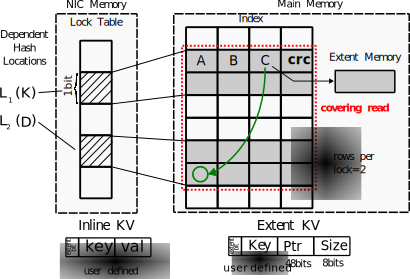
\includegraphics[width=0.99\linewidth]{fig/table-diagram.pdf}
    \caption{Rcuckoo's table design showing an insert of the key $K$ as it displaces $D$.~\todo{add lease table}}
    \label{fig:table-diagram}
\end{figure}



% In this section we describe our protocol for reading,
% inserting, and performing updates and deletes to an rcuckoo
% hash table. Figure~\ref{fig:message_diagram} visualizes our
% protocol.

\subsubsection{Reading} 
\label{sec:reading}

Read requests for key $K$ start by hashing $K$ to calculate
both row locations. Reads are combined if both rows are
within a read threshold to reduce tail latency. We use a
read threshold of 128 bytes as it has a negligible increase
in latency over smaller RDMA
packets~\ref{fig:rdma-benchmarks}(a). If reading both
locations as a single read is greater than 128 bytes, the
read is issued as two parallel reads to individual rows
similar to prior work without locality
optimizations~\cite{pilaf, race}. Inlined entries are read
in a single round trip, while extent entries require two
(Figure~\ref{fig:message_diagram}).

Reads are performed locklessly. Readers recalculate and
check the rows CRC to validate the read. Clients reissue the
read if the CRC is invalid as it is likely due to the read
encountering a torn write. Continuously invalid CRC's can be
the result of a client failure mid write. Our algorithm for
detecting and repairing the table from partially completed
writes is described in Section~\ref{sec:table-repair}.

\subsubsection{Insert}
\label{sec:insert}

Insertions are the highest complexity operation because
client caches are not synced with remote memory. Without
knowing the state of remote memory clients can neither
calculate valid cuckoo paths locally and nor determine which
locks they will require to perform an insertion. We uses a
speculative local search to predict a sufficient set of
locks to complete the insertion and then lock and
synchronize the predicted rows. A second search on the
locked and synchronized rows determines if a valid insertion
path can be found on the locked rows.

\textbf{Speculative Local Search:} The first stage of an
insertion is a speculative local search on the clients
cache. If the client cache is empty a lock for both of the
insertion keys hash locations are made. Otherwise, locks for
each row on the speculative path are acquired. Because of
locality hashing there is a high probability that a valid
insertion path can be found in buckets near a speculative
path, even if the clients cache is stale.

\textbf{Covering Read:} Clients synchronize their local
caches while acquiring speculative locks by reading the rows
the lock protects. These reads are issued in a batch
alongside the MCAS lock request. Speculative locks may not
be sufficient to complete an insertion. However, due to
locality hashing there is a high probability that a valid
path does exist in the neighborhood of the speculative
locks. If two speculatively locked rows are close enough
together clients issus a single \textit{covering read}
spanning both rows. Covering reads populate a clients cache
and dramatically increase the probability that if the first
speculative search fails, a subsequent search will succeed.
We set the max threshold for covering reads to 512 bytes in
all our experiments.  Figure~\ref{fig:table-diagram}
illustrates an insertion of key $K$ displacing key $C$. Here
the speculative search marked the rows for $C$ and $K$ to be
locked. A covering read (red) spans the rows between both
entries.

\textbf{Second Search:} A speculative cuckoo path may be
invalid due to churn in the index. However, as noted their
is high probability that a valid path can be found within
the locked rows due to hash locality. Clients perform a
second search only on the synchronized rows that they have
locked. We use BFS similar to prior work, as it produces
short paths which minimize bandwidth and locking
overhead~\cite{cuckoo-improvements}. If a valid cuckoo path
is found during second search each update and CRC along the
path along with unlock messages are batched together. If no
valid path exists the client releases its locks but retains
its cache. Another speculative search on the fresh cache is
performed. This algorithm is run itteratitivly until a valid
path is found. Our evaluation measures the success rate of
insertions as a factor of lock size
(Section~\ref{sec:search_success}).

During development we
experimented heavily with guided A* search but found that it
only offered improvements over BFS when the table was over
95\% full due to the setup overhead of A* and the fact that
most paths are short.

\subsubsection{Updates and Deletes}

Updates and deletes use an identical message protocol. They
first get both locks for key $K$ while issuing covering
reads (Section~\ref{sec:locking}). If the key is present the
entry is either updated or deleted the version number for
the row is updated and a new CRC is calculated. Both
modifications are issued as separate RDMA writes. For extent
updates new values are batched along with lock requests
preventing an additional round trip. Extent deletes mark the
extent entry for garbage collection.


\subsection{Locality}

\begin{figure*}[t]
    \centering
    \begin{subfigure}{0.3\linewidth}
        \begin{align*}
            L_1 &= h_1(k) \\
            L_2 &= L_1 + (h_2(k)\mod f^{f + log_2(h_3(k))})
        \end{align*}
        % \caption{}
        % \label{fig:hash_factor}
    \end{subfigure}
    \begin{subfigure}{0.3\linewidth}
        \includegraphics[width=0.99\linewidth]{fig/hash_factor.pdf}
        % \label{fig:hash_factor}
        % \caption{}
    \end{subfigure}
    \begin{subfigure}{0.3\linewidth}
        \includegraphics[width=0.99\linewidth]{fig/hash_fill.pdf}
        % \label{fig:hash_fill}
        % \caption{}
    \end{subfigure}.
    \vspace{-1em}
    \caption{
    \textbf{(a)} Dependent hashing for factor $f$.
    \textbf{(b)} CDF of distances between cuckoo locations dependent hashing on different exponential factors.
    \textbf{(c)} Exponential factor relation to max fill in cuckoo hash. 90\% fill marked in red.
    }
    \label{fig:locality-hashing}

\end{figure*}

\begin{figure}[t]
\includegraphics[width=0.99\linewidth]{fig/message_diagram.pdf}
%%
\caption{Rcuckoo's protocol for reads, inserts, deletes and
updates. Blue lines are index accesses, and red lines are
extent accesses. Solid lines are reads, dotted lines are
CAS, and curved dashed lines are writes.}
%%
\label{fig:message_diagram}
\end{figure}

\subsubsection{Dependent Hashing}

Our hashing algorithm borrows from both cuckoo and hopscotch
hashing to achieve constant time reads and a high degree of
locality. The distance between two hash locations is
determined by probabilistically \textit{dependent} rather
than independent hash functions. Dependence makes locality a
tunable parameter. Locality between hash entries reduces the
span of cuckoo paths and increases the probability that both
entries can be read with a single RDMA message. However,
high locality increases the probability of hotspots in the
table which decreases its maximum fill factor.

Figure~\ref{fig:locality-hashing}(a) is our formula for dependent
hashing. The first hash location is chosen uniformly at
random, while second is chosen as an offset of the first.
$f$ determines the max distance the second item can be
placed. Higher values of $f$ decrease locality.
Figure~\ref{fig:locality-hashing}(b) shows the distance between hash
locations as a CDF for different values of $f$. Setting a
constant bound on the distance between hash locations leads
to bad fill factors (on the order of 10-15\%). Our function
places exponentially few locations exponentially far apart
using a third hash function $h_3(x)$ which generates a
higher exponent at a logarithmic rate to determine which
locations will have large distances between
them~\footnote{The value of $h_3(x)$ is the sum of trailing
zeros after calculating a keys 64bit hash value} These few,
but far apart hash locations increase the max fill by
alleviating hotspots in the table. During inserts these
entries act as gateways for search to access less filled
portions of the table. 

Figure~\ref{fig:locality-hashing}(c) shows how larger values of $f$
enable higher fill factors for tables with 100M entries.  In
our experiments we use $f$ of 2.1 and an associativity of 8
as it provides a 90\% max fill an a 68\% probability that
hash locations are located 3 or fewer buckets apart.


\subsubsection{Locking}
\label{sec:locking}

\begin{figure*}[t]
    \centering
    \begin{subfigure}{0.3\linewidth}
        \includegraphics[width=0.99\linewidth]{fig/optimistic_failures.pdf}
        % \label{fig:optimistic_failures}
        % \caption{}
    \end{subfigure}
    \begin{subfigure}{0.3\linewidth}
        \includegraphics[width=0.99\linewidth]{fig/insertion_span.pdf}
        % \label{fig:insertion_span}
        % \caption{}
    \end{subfigure}
    \begin{subfigure}{0.3\linewidth}
        \includegraphics[width=0.99\linewidth]{fig/buckets_per_lock_vs_locks_per_message.pdf}
        % \label{fig:tbd}
        % \caption{}
    \end{subfigure}
    \vspace{-1em}
    \caption{
    \textbf{(a)} Failure rate of optimistic cuckoo insertions.
    \textbf{(b)} CDF of cuckoo spans for dependent and independent hashing. A cuckoo span is the distance between the smallest and largest index in a cuckoo path.
    \textbf{(c)} Round trips (99th percentile) on a table
    with 512 rows required per insert while filling a table
    to 95\%. 512 buckets per lock is a single global lock.}

    \label{fig:cuckoo-problems}

\end{figure*}

Using locks rather than opportunistic concurrency halves the
latency of reads from two to one round trip. Opportunistic
updates commit changes by atomically updating a pointer
(with CAS) in the hash index to point to a new value. Both
the index, then the value must be read for each operation.
Values can not be inlined in the index as they are limited
to the 64bit width of CAS. Rcuckoo uses locks to enable
inlined entries which can be read in a single round trip.
Locks introduce multiple challenges such as scalability,
deadlocks and fault tolerance each of which is discussed
below.

RCuckoo uses hardware NIC hardware features and lock
virtualization to achieve scalability, low contention and
high performance. The lock table is a linear array of bits
where 1 is locked, and 0 is unlocked. Each bit locks one or
more contiguous rows in the table. In our experiments we use
16 rows per lock as it has a negligible effect on contention
and requires a single lock to be acquired for \todo{85\%
double check} of insertions.

We use two RDMA NIC features to accelerate lock
acquisition. First the lock table is placed in NIC device
memory which allows atomic operations (CAS) to
scale linearly with reads and writes and is 3x higher
throughput on contented addresses than host memory (see
Figure~\ref{fig:rdma-benchmarks}). It is also lower latency
as operations to device memory avoid a PCIe round trip.
Second, RDMA Masked Compare and Swaps (MCAS) are used rather
than CAS~\cite{rdma-masked-cas,sherman}. CAS requires an
exact 64 bit match to execute, while MCAS uses a mask to
only set the required bits. MCAS therefore reduces
contention while enabling locks to be as tightly packed.

Packing locks densely is important as NIC device memory is
limited to 256KB which by default limits table size. We use
a \textit{virtual lock table} to avoid limiting table size
by device memory.  Multiple virtual locks map to a single
physical lock. We use modulo arithmetic to map virtual locks
onto physical lock to support arbitrarily large tables.
Mapping multiple virtual to a single physical lock leads to
false sharing, clients can be blocked unessisary on a lock.
In Section~\todo{TODO} we show that on large lock tables the
performance degradation due to false sharing is low, and
that lock locality is maintained on virtual locks.

Our deadlock free locking protocol acquires and releases
locks in order.  Given a list of virtual locks to aquire a
client calculates their physical locations and sorts them.
The sorted locks are broken into 64 bit chunks which are
mapped to individual MCAS packets. As shown in
Figure~\ref{fig:cuckoo-problems}(b) 99\% of insertions are
within a 256 bucket range. Each MCAS covers 1024 buckets so
the common case is a single chunk. Lock requests are issued
in order. Clients continuously poll on lock requests and
only move to the next request only after the prior has been
successfully acquired.

Clients may fail while holding locks leaving them set and
stranded. Clients detect failed locks by timing out on them
while acquiring them. To separate failures from clients
acquiring a long list of contended locks clients are given a
bounded time to aquire their locks. If a client takes longer
than this time to aquire all of its locks it releases all
held locks and starts the process again to prevent false
failure detection. Our complete fault detection and recovery
mechanism is described in Section~\ref{sec:fault-tolerance}.

\subsection{Fault Tolerance}
\label{sec:fault-tolerance}

The table must be repaired if a client fails while holding a
lock. In our fault recovery algorithm non-failed clients
aquire repair leases to reclaim the locks of failed clients
and then perform the operations required to return the table
to a valid state. In this section we describe how RCuckoo
clients detect faults, repair the table, and prevent stray
RDMA writes from failed clients from corrupting the table.

\subsubsection{Failure Detection} 
\todo{note that we don't know who has the lock or when they got it}

Clients detect failures with timeouts triggered when a lock
acquisition or read fails repeatedly and the state of the
locked or read rows is unaltered by other clients.  True
failures are distinguished from frequently accessed rows by
checking CRCs which are modified on every row update due to
row version numbers (Section~\ref{sec:table-design}).
Clients reset their failure timers whenever a CRC changes
between requests.


\todo{talk about the actual timeout value} We view failures
as a rare but essential component of our protocol. As such
our fault timers are set conservativly. Failure timers for
locks must include locking time, second search time, and
update transit time. We bound locking time (Section
~\ref{sec:locking}), search, and message propagation is
measured in single digit microseconds. We additionally want
to ensure that network conditions are not causing continual
RDMA retries. We set the max RDMA operation retry number to
3 for all our experiments. We set our failure timeout to
100ms as it is orders of magnitude above our 99th percentile
insert time (50us) and above the RDMA retry limit.


\subsubsection{Repair Leases}
\todo{mention repair lease table}

Repair leases provide clients with exclusive permission to
reclaim locks on a region of the table. The table is broken
into $n$ regions so repairs can be executed in parallel (see
Figure~\ref{fig:table-diagram}). Leases are set with 64 bit
CAS and track the lease holders QP id, a set bit, and a
counter (incremented on each acquisition).  Failures while
holding a lease are easier to detect than normal locks as a
leases owner and liveness are tracked within it.  Leases are
revoked using a similar timeout to normal locks. When a
client times out on a lease it claims it for itself and
marks the lease holder as failed (see
Section~\ref{sec:stale-writes}).  A lock is reclaimed once a
client both times out on a lock and acquires the locks
repair lease. 


\subsubsection{Table Repair} 
\label{sec:table-repair}

Cuckoo updates occur along a path
and client failures could occur at any point along an
insertion path. Updates and Deletes are a special case where
the path length is 1. If a client fails mid modification it
can leave the table in 3 distinct states based on where in
the update it fails. 

Our table design ensures that clients can perform repairs
and recover from all states a failed client may have
created. Recovery is simple if a client with locks fails
prior to issuing its updates or if it fails before releasing
its locks. A client with a repair lease can simply set
unlock the stranded lock in this case. Failures during
modifications require special care to recover from. All
modification operations Update, Delete, and Insert write new
entries as a cuckoo path~\footnote{updates and deletes are a
cuckoo path of length 1}. As described in
Section~\ref{sec:insert} cuckoo paths are executed by first
setting an open entry to claim it and migrating entries
backwards along the path until a new entry is written. If
partially executed this algorithm can produce 3 distinct
states.

\begin{enumerate}
    \item{A duplicate entry exists and one has a bad CRC}
    \item{A duplicate entry exists and both have correct CRCs} 
    \item{No duplicate exists but one row has a bad CRC}
\end{enumerate}

To repair the table a client first detects which state the
table is in and then transitions the table forward through
the states with a deterministic sequence of operations so
that failures during recovery can be continued by any other
client. A client detects the state issuing reads to all rows
protected by the stranded lock. Then all entries within the
rows have both hash locations read individually to check for
duplicates. The error state can be detected by the presence
of duplicates in these rows and the existence of bad CRCs.

Table corrections are issued as a batched sequence of 3 or
fewer writes as follow: $1 \rightarrow 2$ - write a new CRC
for the bad duplicate.  $2->3$ - Set the duplicate in the
second hash location to empty. $3\rightarrow$ - recalculate
and write a new CRC. After a client has issued its repair
sequence it unlocks the reclaimed lock and returns its
lease.


\subsubsection{Preventing Stale Writes}
%%
\label{sec:stale-writes}
%%

An RDMA connection must be closed, transitioned to an error
state, or have it's permissions revoked to prevent its
operations from being executed on memory. Because we assume
remote memory is passive (it will not tear down connections)
and that faulty clients will not tear down their connections
it is possible that the connection of a failed client will
stay open and stale writes may be delivered to memory after
a faulty clients lock is revoked. We use conservative
timeouts to out-wait network delays and RDMA retransmissions
at the cost of recovery latency. 

At the time of writing the infiniband specification does not
enable clients to modify each others permissions. Type II
memory windows enable clients to remove their own
permissions using the \textit{send with invalidate} verb. If
the specification were extended to allow a client with
elevated privileges to revoke the permissions of a faulty
client it would provide a clean means of handling client
failure in the disaggregated setting. Given the current
specification a client can corrupt the QP's of another by
sending a crafting an invalid packet and sending to their
queue pair pair~\cite{redmark}[attack 2]. For this attack to
work the packet sequence number of the shutdown packet must
match the sequence number of the receiver so $2^{24}$
packets must be sent to ensure a connection is corrupted
successfully.

\section{Implementation}

We implement our algorithm in
Python and emulate client-based RDMA using a custom-built
simulator consisting of 1k lines of code. 

\textbf{Simulator:} Our simulator is event based and does
not emulate network transit time, processing time, or failed
packets. Clients, memory, and switches are modeled as finite
state machines, and the network as FIFO queues. Events are
scheduled randomly, multiplexing clients, memory, and the
network. RDMA verbs are modeled as function pointers with
arguments passed by the client.

\textbf{Rcuckoo} is implemented in 1.2k lines of
python. We implement our own version of approximate A* with
the use of Python's standard heap library for priority
queuing. Clients store complete copies of the remote hash
table index locally. We do not model the hash table extent
in simulation all table accesses are inlined. In practice
for better resource utilization cached pages of the index
could be released using LRU. 

\textbf{RACE~\cite{race}} has no publicly available
implementation. Therefore we implemented our own version of
RACE by closely following its protocol as described in its
paper.  We only model the RACE index. In cases where
blocking calls are made to RACE's extent we assume they
succeed and simply reissue a read to the index to model the
round trip incurred by the extent lookup. We model RACE's
blocking behavior exactly in this way. We reached out to
RACE's authors to check our implementation's correctness and
were able to correlate our fill factor results with theirs.

\section{Evaluation}
\label{sec:eval}

We evaluate RCuckoo by directly comparing its performance in terms of
throughput and latency against representative state-of-the-art
disaggregated key/value stores and find that RCuckoo outperforms them
all in terms of throughput while delivering competitive insert
latencies.  Using fault injection, we show that our distributed
approach to client failure detection and recovery enables RCuckoo to
sustain high throughput even though 100s of clients are failing per
second.  Finally, we justify our design decisions through a series of
micro-benchmarks. Specifically, we quantify the benefit RCuckoo
extracts from its locality enhancement and speculative search strategy
and conduct sensitivity analyses of our choice of locality parameter,
covering read threshold, and index-table entry size.

\section{Implementation}

We implement our algorithm in
Python and emulate client-based RDMA using a custom-built
simulator consisting of 1k lines of code. 

\textbf{Simulator:} Our simulator is event based and does
not emulate network transit time, processing time, or failed
packets. Clients, memory, and switches are modeled as finite
state machines, and the network as FIFO queues. Events are
scheduled randomly, multiplexing clients, memory, and the
network. RDMA verbs are modeled as function pointers with
arguments passed by the client.

\textbf{Rcuckoo} is implemented in 1.2k lines of
python. We implement our own version of approximate A* with
the use of Python's standard heap library for priority
queuing. Clients store complete copies of the remote hash
table index locally. We do not model the hash table extent
in simulation all table accesses are inlined. In practice
for better resource utilization cached pages of the index
could be released using LRU. 

\textbf{RACE~\cite{race}} has no publicly available
implementation. Therefore we implemented our own version of
RACE by closely following its protocol as described in its
paper.  We only model the RACE index. In cases where
blocking calls are made to RACE's extent we assume they
succeed and simply reissue a read to the index to model the
round trip incurred by the extent lookup. We model RACE's
blocking behavior exactly in this way. We reached out to
RACE's authors to check our implementation's correctness and
were able to correlate our fill factor results with theirs.


\begin{figure*}[ht]
    \includegraphics[width=0.99\linewidth]{fig/hero_ycsb_throughput.pdf}

    \caption{Throughput as a function of the number of clients for three different workloads (Zipf $\theta$=0.99): \textbf{(a)} YCSB-A 50\%
    read 50\% update, \textbf{(b)} YCSB-B 95\% read 5\% update and \textbf{(c)}
    YCSB-C 100\% read.}
    \label{fig:ycsb_throughput}
 \end{figure*}


\subsection{Testbed}

We conduct our evaluation on an 11-node cluster of dual-socket Intel
machines. Each CPU is an Intel Xeon E5-2650 clocked at
2.20~GHz. Each machine has 256~GB of RAM with 128~GB per NUMA
node. All machines have a single dual-socket ConnectX-5 attached to a
100-Gbps Mellanox Onyx switch. In our RCuckoo experiments we use one
sever as the memory server and the rest a client machines
spreading threads evenly across machines.

%\subsection{Comparison systems}

We compare RCuckoo against three recent RDMA key-value stores with
different designs, FUSEE~\cite{fusee}, Clover~\cite{clover}, and
Sherman~\cite{sherman}.  While none have the exact same assumptions or
feature set as RCuckoo, each represents an apt comparison point for
different aspects.  To avoid biasing our evaluation, we use the same
workloads (YCSB) as the previous efforts.
%
%We directly compare RCuckoo against three disaggregated
%key-value stores  Each system has distinct design
%tradeoffs. 
%%
%%
%%

\textbf{FUSEE} is a fully disaggregated key/value store that
represents the closest available comparison point to RCuckoo.  While
both employ only 1-sided RDMA operations, FUSEE eschews locking in
favor of optimistic insertions.  FUSEE clients use CAS operations
to manage fixed, 64-bit index table entries that contain pointers to
values stores in extents.  Due to its reliance on CAS operations, FUSEE is unable to support inlined storage of small
values like RCuckoo, forcing all reads to require two round trips.
%Fusee is the closest comparison we have to illustrate
%the tradeoffs between locks and optimistic concurrency.
%is a key-value store designed for full
%disaggregation~\cite{fusee}.  It is built on top of RACE~\cite{race}
Unlike RCuckoo, FUSEE is designed to support replication.  To remove the overhead of replication, 
%While RACE represents a more direct comparison to RCuckoo, no open
%source implementation of RACE is available.  Instead,
we deploy FUSEE with a single memory node.
%FUSEE/RACE hashing uses fixed-sized 64-bit index entries
%to in order to employ RDMA compare-and-swap operations for updates. As
%such, RACE-based systems cannot store key-value pairs in the index
%table itself and require a second round trip even for reads of small values.
%on reads to recover
%extent entries which contain full key value pairs.

\textbf{Clover} is only partially disaggregated---it requires a
metadata server to manage its index structure---but can deliver higher
read performance than FUSEE on read-only workloads.  Clover is
designed to leverage remote persistent memory and implements both
reads and updates using one-sided RDMA operations.  Moreover, unlike
FUSEE---and similar to RCuckoo---Clover reads are self verifying.
%Clover uses index caching to optimize reads.  When re-reading key-value
%entires clover can as it directly
%reads the entry without negotiating with the index.
In contrast to prior Clover comparisons~\cite{fusee} that force
clients to consult the metadata server on each read, we allow Clover
to take advantage of its client caching to achieve maximum performance
on read-heavy workloads.

%% Clover is a partially disaggregated system which uses
%% two-sided RDMA operations to modify the index and one-sided
%% operations for updates, deletes, and reads.

%% Sherman a disaggregated B-Tree and the only system at the
%% time of writing which uses locks and not optimistic
%% concurrency to guard its index. Our performance comparison
%% with Sherman is not apples to apples. Sherman maintains
%% ordered key-value pairs for range queries and thus has
%% higher overheads on updates than the other systems.

\textbf{Sherman} is the highest-throughput distributed key/value
storage system of which we are aware that employs locks.  Sherman
maintains a B-tree that spans multiple servers and supports range
queries, a feature none of the other systems---RCuckoo
included---provide.
%is a B-tree designed for remote memory~\cite{sherman}.
%and high write
%throughput.
%Unlike Clover and FUSEE which employ optimistic consistency control,
%Sherman uses locks to guard updates similar to RCuckoo.
On the other
hand, Sherman clusters are not fully disaggregated: each node in a
cluster is a peer with many CPU cores and a single memory core
that is responsible for servicing allocation RPC calls from clients.
%Unlike the other systems
%Sherman is cluster based, and does not support a having
%isolated memory machines.
%All machines are equal nodes in a
%cluster and run both a memory controller and client threads.
As such, Sherman does not encounter the same bandwidth bottlenecks as
the other systems because requests are partitioned across all
machines in the cluster.
%However, it assumes that collocated clients can resolve lock
%contention locally and clients collocated with their segment
%of the B-Tree can perform local operations. These
%assumptions enable Sherman to have high performance under
%contention even though it uses locks and manages a more
%complex data structure than the unordered key-value stores.
%While Sherman does not meet the fully disaggregated model it
%does provide a good comparison for RCuckoo as it is the only
%other system to use locks in remote memory.


% \subsubsection{Clover}
% \todo{insert a short clover description}

\begin{figure*}[ht]
    \includegraphics[width=0.99\linewidth]{fig/hero_ycsb_fill.pdf}

    \caption{Performance as a
    function of fill factor. \textbf{(a)} Throughput for four different YCSB insert workloads, \textbf{(b)}
    median operation latency, \textbf{(c)} mean operation size, and \textbf{(d)}
    mean RDMA message count per operation under YCSB-A.}

    \label{fig:ycsb_fill}
\end{figure*}

% \begin{figure}[ht]
%     \includegraphics[width=0.99\linewidth]{fig/hero_ycsb_fill_ops_bw.pdf}
%     \caption{YCSB-A workload messages and bandwidth per operation as a function of fill factor}
%     \label{fig:ycsb_fill_ops_bw}
% \end{figure}



\subsection{Performance}

We start by considering the classical YCSB workloads which employ
varying mixes of read and update operations before turning to the more
complex insert operation.  RCuckoo delivers the highest performance
across all settings, while the others each shine on different
mixes.

\textbf{YCSB:}
Figure~\ref{fig:ycsb_throughput} shows throughput in terms of
operations per second for RCuckoo, FUSEE, Sherman, and Clover on
three different YCSB workloads with a Zipf(0.99) distribution. YCSB-A
is a 50\% read 50\% update, YCSB-B is 95\% read and 5\% update, and
YCSB-C is 100\% read.  In each experiment a variable number of clients
insert 90-M entries containing 32-bit keys and 32-bit values into a
100-M-entry hash table.


On YCSB-A RCuckoo begins to surpass FUSEE after about 125 clients.  FUSEE's maximum performance is gated by its requirement for an additional round trip per operation (to
retrieve the extent). Sherman keeps pace until about 5 MOPS at which
point it suffers from lock contention due to its B-Tree structure.
(Sherman and RCuckoo perform similarly for uniform workloads where
lock contention is less of an issue.).  Clover performs the worst
under write-heavy workloads due to its inability to effectively leverage
client-side caching of a constantly changing index structure.

On read-mostly and read-only workloads (YCSB-B and C)
RCuckoo extracts even further benefit over FUSEE from its ability to
complete read in a single round trip rather than two and gains
additional benefit by collapsing most reads into a single packet
(Section~\ref{sec:read_threshold}).  Sherman performs well on
read-mostly workloads as it can directly read from the B-Tree in a
single round trip without the need for pointer chasing, but it
continues to bottleneck on lock contention in YCSB-B due to hot
keys. While Sherman experiences no such bottleneck on YCSB-C its read
algorithm is more complex than RCuckoo's leading to lower top-end
performance. Clover performs similarly to FUSEE on YCSB-B, and is the
most competitive with RCuckoo in read-only scenario.  When it is able
to leverage its client index cache, Clover's reads are very similar to
RCuckoo in that they require only a single 1-sided RDMA read;  we
suspect that with tuning Clover's read-only performance
could be brought to par with RCuckoo.

\textbf{Inserts:}
%%
%By default YCSB-A,B,C use updates. RCuckoo's insert
%algorithm is it's most complex and bandwidth intensive
%component. In this section
Despite its complexity, RCuckoo's insert operation remains highly
performant.  To evaluate insert performance we modify YCSB to perform
inserts rather than updates.  Figure~\ref{fig:ycsb_fill} considers
RCuckoo's performance on workloads that exclusively use inserts (rather than
updates), for example in this instance YCSB-A is 50\% insert and 50\%
read. YCSB-W is write only, i.e. a 100\%-insert workload.  Inserts become
more expensive as the table fills, so we report insert performance as
a function of the table's fill factor.

Figure~\ref{fig:ycsb_fill}(a) shows the aggregate throughput
of 400 clients across four different workloads as a function
of the table's fill factor.  As the index table fills,
cuckoo paths become longer leading to increased contention
and additional bandwidth consumption from larger covering
reads. In each case (except YCSB-C) RCuckoo's performance
declines with fill factor. In the insert-only YCSB-W case
RCuckoo's performance drops from 11.5 to 4.5 MOPS.  As a
point of comparison, FUSEE's maximum insert-only performance
is 9.1 MOPS on our testbed, although it is independent of
fill factor.  While FUSEE out-performs RCuckoo at high fill
factors, we observe that an insert-only workload is uncommon
in practice~\cite{facebook-memcached}.

We plot operation latency, size, and message counts (in
terms of RDMA packets) as a function of fill factor in
Figure~\ref{fig:ycsb_fill}(b--d).  For comparison, we report
latency values of insert and read operations for the
comparison systems. These values were not collected under
load and represent best-case performance on our testbed.
Read latency is nearly identical for all systems save FUSEE,
as it requires an additional round trip.  Insert times vary:
Clover and Sherman use two-sided RDMA operations for insert
and both need to perform allocations and set up metadata for
the requesting client.  FUSEE is slightly slower, roughly
the same as RCuckoo's best case.  As the table fills,
however, cuckoo paths grow in length causing RCuckoo insert
operations to require additional round trips to find valid
cuckoo paths.  At maximum fill, insert operations take
roughly twice as long as in an empty table. This rising costs
is reflected by the increase in both bytes (Figure~\ref{fig:ycsb_fill}(c)) and messages (Figure~\ref{fig:ycsb_fill}(d)) per
operation.  RCuckoo reads, on the other hand, have roughly
the same cost and performance regardless of fill factor.


\begin{figure}[t]
    \includegraphics[width=0.99\linewidth]{fig/fault-rate.pdf}
    \caption{Throughput vs failure rate.}
    \label{fig:failure_throughput}
    \vskip -1em
\end{figure}

\subsection{Fault tolerance}

RCuckoo runs at nearly full throughput during realistic
failure scenarios and remains functional in the face of
hundreds of failures per second. When a client fails while
holding a lock the lock is stranded and requests for that
lock will block until after a client times out and reclaims
the lock.
%%
We emulate hundreds of client failures per second by
performing a partial insert operation which truncates the
batch of insert packets including lock releases. The table
entries are left in one of the inconsistent states listed in
Section~\ref{sec:table-repair} and locks are left set.


Figure~\ref{fig:failure_throughput} illustrates RCuckoo's
ability to operate at high throughput in the face of
failures. Lock granularity increases the probability that
multiple clients will block on the same failed lock. Larger
locks have little difference when failures are semi-frequent
and have a larger impact as hundred of failures occur per
second.  The performance impact of a few number of failures
per second is low which is ideal considering that failures
in RDMA clusters are relatively rare.  As a point of
reference, we observe that RCuckoo can still operate despite
thousands of failures per second while a server can only
establish approximately 1.4~K RDMA connections per second
using state of the art techniques~\cite{xrdma}.

\subsection{Microbenchmarks}

Having established RCuckoo's superiority over prior systems and
demonstrated its robustness to client failure, we now evaluate the
impact of particular design choices.

\subsubsection{Locality enhancement}

\begin{figure}[t]
    \includegraphics[width=0.99\linewidth]{fig/search_dependence.pdf}

    \caption{Round trips per insert operation with independent
    and dependent hashing.  (Note log-scale axes.)}

    \label{fig:search_dependence}
\end{figure}

%Hash dependence and search function choice have the highest
%impact on RCuckoo's performance. Dependent hashing reduces
%the probability locks are scattered throughout the table
%which enables RCuckoo to combine lock requests into a few
%masked CAS messages. Simultaneously search function choice
%dramatically affects the length of cuckoo paths.

Figure~\ref{fig:search_dependence} illustrates the dramatic benefit
RCuckoo extracts from its dependent hashing combined with a BFS
cuckoo-path search strategy.  To focus on longer cuckoo paths, we
pre-fill a 100-M entry table to 85\% and then report both the median
and 99th percentile number of round trips required to insert new
key/value pairs until the table is 95\% full as a function of lock
granularity.  While median performance is on the same order, the
99th-percentile insert takes an order of magnitude fewer round trips
with dependent hashing and BFS as opposed to independent hashing and
DFS as used in prior cuckoo hash
systems~\cite{cuckoo-improvements,pilaf,cuckoo}.  As before
(c.f. Figure~\ref{fig:cuckoo-problems}), performance is similar with
four or more locks per message.

%% We vary the number of locks per message to demonstrate the
%% effect of path length and show why masked cas plays an
%% important role in RCuckoo's performance. We measured both
%% the median, and 99th percentile round trips per request on a
%% table with 100M entries. We fill the table to 85\% and then
%% executed insert operations to 95\%.

%% DFS with no hash dependence has extremely poor performance
%% at it's tail, taking over 2K round trips to complete. Both
%% at it's median and 99th percentile it sees only small
%% benefits from setting multiple locks per request as the
%% locks are scattered throughout the table. DFS with
%% dependence has far lower tail latency, and improves the
%% number of locks which can be acquired per message, however
%% it still constructs long rather than minimum length paths.
%% BFS with dependence provides the best performance and gains
%% the most from setting more locks per request. At 64 locks
%% per request it has 7.5x lower round trips at it's 99th
%% percentile and 4 rather than 5 round trips on average. We
%% found that A* search provided the same minimal path length
%% as DFS with slightly better locality. It's performance
%% against BFS was only superior at fill factors above 95\% and
%% lower elsewhere due to a higher runtime cost on short paths.



% Hash function locality hash a major impact in RCuckoo's
% performance.  Acquiring locks can only be done in a few
% round trips when the locks are clustered together tightly in
% the lock table.  Furthermore, the search function used to
% determine the cuckoo path has a large impact on the locality
% of the locks necessary to lock the path. We evaluate
% dependent hashing and independent hashing as well as random
% and a* search. We measure the number of round trips required
% for each control as a function of the number of locks which
% can be acquired per round trip.

% Figure~\ref{fig:search_dependence} shows the performance
% improvements gained by both locality hashing and A* search.
% In this experiment the table is filled from 0 to 90\% full
% with a YCSB-w workload. We measure the 99th percentile of
% round trips for these workloads. Random search with
% independent hashing leads to a large number of round trips
% as locks are scattered throughout the table. RDMA masked CAS
% operation do little here to reduce the round trips as they
% can rarely acquire more than one lock in a round trip. With
% dependent hashing and random search RDMA CAS operation are
% almost sufficient to reduce round trips, however the absolute
% number of locks required per insert is high which leads to
% greater contention. A* search with dependent hashing has
% cuckoo paths that are both short, and clustered together.


\subsubsection{Speculative search}

\label{sec:search_success}
\begin{figure}[t]
    \includegraphics[width=0.99\linewidth]{fig/search_success_lock_size.pdf}
    \caption{Failure rate of search algorithms vs lock size under high contention}
    \label{fig:search_success}
\end{figure}

RCuckoo's two stage search algorithm is designed to improve
the probability that an insert will be successful given that
a clients local cache is out of sync. To demonstrate the
effectiveness of our two stage search strategy we measure
the success rate of our searches under high contention. With
400 concurrent clients we fill a small table (10M entries)
up to 85\% prior to measuring success rate in order to
maximize cuckoo path length. Figure~\ref{fig:search_success}
shows the failure rate of both search stages. The first
search is the success rate of a search based entirely on
cached information. The second search is the success rate of
our restricted search performed after acquiring locks. We
measure the response of both as a function of lock size.
Given 1 row per lock the failure rate of both searches is
over 4 as the local cache is almost always out of sync, and
retries are not guaranteed to be synchronized. As lock
granularity grows the frequency of second search success
drops dramatically. At 64 rows per lock our second search
succeeds 95\% of the time even when the cached search fails
at a rate of 99\% per insert.


\begin{figure*}[t]
    \centering
%    \begin{subfigure}{0.3\linewidth}
%        \includegraphics[width=0.99\linewidth]{fig/masked_cas_lock_size.pdf}
%    \end{subfigure}
    \begin{subfigure}{0.3\linewidth}
        \includegraphics[width=0.99\linewidth]{fig/factor.pdf}
        % \label{fig:hash_fill}
        % \caption{}
    \end{subfigure}
    \begin{subfigure}{0.3\linewidth}
        \includegraphics[width=0.99\linewidth]{fig/read_size.pdf}
        % \label{fig:hash_factor}
        % \caption{}
    \end{subfigure}
    %\begin{figure}[ht]
    \begin{subfigure}{0.3\linewidth}
      \includegraphics[width=0.99\linewidth]{fig/entry_size.pdf}
          \end{subfigure}
%    \caption{Throughput vs KV entry size}

%\end{figure}
    \vspace{-1em}
    \caption{RCuckoo parameter sweeps:
      \textbf{(a)} Throughput and max fill vs locality factor,
          \textbf{(b)} throughput vs read threshold, and 
    \textbf{(c)} throughput vs key/value entry size.
    }
    \label{fig:performance_breakdown}
             \label{fig:entry_size}
\end{figure*}

%% \subsubsection{Masked CAS}

%% Under contention masked CAS operations provide a significant
%% performance improvement. We measure it's benefit in terms of
%% throughput by comparing it with default CAS. In the
%% default case, when acquiring locks clients set the lock bits
%% for the locks they require and set all other bits in the cas
%% to 0. If the cas fails the current state of the lock table
%% over that range is returned as a result to the client and
%% the client tries to acquire their locks again using the
%% updated state of the lock table. Masked compare and swaps
%% are issued with the minimal mask required to set the locks.

%% Figure~\ref{fig:performance_breakdown} shows the improvement
%% gained by masked CAS. Default CAS operations perform better
%% with fewer rows per lock, as the probability of a lock being
%% set within the 64bit range is at its lowest. At higher rows
%% per lock CAS suffers from failed lock acquisitions from both
%% contested locks and due to a lack of synchronization. In
%% contrast masked CAS sees an improvement when two rows per
%% lock are used, as more second search attempts succeed, and
%% only suffers from direct lock contention as the rows per
%% lock increase.


\subsection{Parameter sweeps}

Figure~\ref{fig:performance_breakdown} plots the sensitivity of
RCuckoo performance to various parameter settings.

\textbf{Locality factor.}  The left-most graph shows that lower hash
factors $f$ deliver higher performance (plotted against the left axis)
due to better locality at the cost of lower expected maximum fill
factors (right axis).
%the tradeoff of their maximum fill factor. The
%relationship between $f$ and performance is nearly linear, while the
%relationship between $f$ and fill factor is
%exponential. Figure~\ref{fig:performance_breakdown}(c) shows the
%relationship between $f$, the max fill rate, and insert
%performance. These numbers were collected on an
This experiment consists of an insert-only workload (YCSB-W)
on a 100-M entry table. We choose an $f$ of 2.3 in practice as
it has the highest product of fill factor and throughput.
\todo{Section 4 says we use an f of 2.1?}

\textbf{Read threshold.}
\label{sec:read_threshold}
As described in Section~\ref{sec:reading} RCuckoo issues a covering
read if both key locations are within a defined threshold (128 bytes
in our experiments) of each other.
Figure~\ref{fig:performance_breakdown}(b) shows that performance
increases with larger thresholds, but at the cost of additional
bandwidth consumption.  In this experiment, only 40 clients
access a table with 64-byte rows, so they do not exhaust link bandwidth even with a 4-KB covering read, but performance levels off after 2 KB.
%% performance gains from increasing the read threshold. Here
%% each row is 64 bytes so our minimum threshold of 64 ensures
%% two packets are issued for each read request. We limit the
%% number of clients to 40 so that their is plenty of bandwidth
%% to support the inflated reads. Higher read thresholds trade
%% off network bandwidth for operation latency. 
Under these conditions, if bandwidth is plentiful larger (i.e., 2-KB
vs 128-B) covering reads can improve throughput, but only modestly.
%8\%.

% \begin{figure}[ht]
%     \includegraphics[width=0.99\linewidth]{fig/read_size.pdf}
%     \caption{Read Threshold vs Throughput}
%     \label{fig:read_threshold}
% \end{figure}


\textbf{Entry size.}  Inlined key/value entries enable RCuckoo's
single-round-trip reads, so the larger the entries, the fewer values
that require a second round trip.  However, for a fixed row size,
larger entries imply fewer entries per row, increasing cuckoo path
lengths (when measured in terms of rows), impacting insert performance.
%% but larger values must be stored in extents.  
%% at the cost of inflating the bandwidth of
%% operations. We run a 50\% read 50\% insert and a read only
%% workload to illustrate the overhead of larger entries.
Figure~\ref{fig:entry_size}(c) shows the effect of entry size on
operation throughput under YCSB-A. Insert is a bandwidth-limited
operation;
%quickly saturates
%the network bandwidth. At
at 16-B entries link capacity restricts throughput to 8 MOPS. The
performance of reads (and updates/deletes, not shown), on the other
hand, are largely unaffected by entry size.  Hence,
%which have lower
%bandwidth requirements see very little chance in throughput
%across entry sizes. We suggest that known read heavy
%workloads should use inlined entries as reads see a large
installations serving read-heavy workloads may wish to favor larger entry sizes.
%
%boost in performance. Update operations are similarly
%unaffected by entry size up to 64 bytes. 

% Our design choice
% in embedding KV pairs is motivated by networking trends
% which suggest that 800 GBPS and higher network speeds will
% be available in the coming years. While round trip latency
% is expected to remain largely the same.





\section{Limitations}
\label{sec:limations}

\subsection{replication and persistance}
At the time of writing Rcuckoo does not support multiple
memory nodes for replication and is not designed for
persistance. No aspect of RCuckoo's algorithm prevents the
use of multiple replicas. As Rcuckoo uses lock based
protection, replicated updates can be broadcast by writes to
each replica prior to releasing locks. Rcuckoo's index is
not designed for persistance. As Rcuckoo is primarily an
index, we see it as compatable with the persistance
strategies of other disaggregated projects. For instance
RCuckoo could easily make use of Clover's persistent extent
algorithm with no changes to RCuckoo's index structure.

\subsection{Replication, and scalability} 
\todo{no real replication probabily delete, consider moving
to future work / limiations} At the time of writing RCuckoo
does not support replication although replication is in no
way a complication for our existing algorithms. On inserts
clients aquire locks from a master memory node as described
in section~\ref{sec:insert}, after locks are acquired on the
master node updates, deletes, or cuckoo paths are broadcast
to replicas. Replication requires a clients to wait for
responses from replicas before issuing unlock messages as
the client can not rely on RDMA RC connection in order
delivery across the multiple replica connections.

\todo{We don't span multiple memory nodes} When using
multiple memory machines each machine is initialized with an
equal portion of the cuckoo index and lock table. Clients
calculate which machine to issue their requests to when
generating requests.


\subsection{Client Scalability} RCuckoo's algorithm relies
on the semantics of in order delivery for the correctness of
it's locking and reading algorithms. RDMA NIC's have hard
caps on the number of reliable connections they support
~\todo{(~65k)} these limitations are fundamental to the
cache size on the RDMA NIC~\cite{erpc,faast}, although cache
sizes have steadily increased~\cite{storm}. RDMA unreliable
connections currently do not support one-sided verbs making
them unusable for disaggregated applications.

\section{Conclusion}
\label{sec:conclusion}

In this work we design and implement a lock-based cuckoo hash table
for passive remote memory. Using dependent hashing, a carefully
designed locking protocol, and the latest RDMA NIC features we achieve
single-round-trip reads, update operations that require two round
trips when uncontested, and insert operations that require only two
round trips in the median case.  Even in the face of high contention
and nearly full tables, client caching limits I/O amplification.
Moreover, our step-by-step insert protocol enables fully disaggregated
failure detection and recovery.  Future work could consider employing
a data replication strategy that addresses server failure in a
similarly disaggregated manner.


\section*{Acknowledgments}

Thanks for everyone that supported me. Thanks to Pengfei Zuo
for assistance in replicating results from the original RACE
paper.


\balance
\vspace{-0.3cm}
{\footnotesize \bibliographystyle{acm}
\bibliography{paper}}
\vspace{-0.5cm}

\end{document}
